\graphicspath{{4int/asy/}}

\section{Integration}

The theory of infinite series addresses the problem of summing infinitely many \emph{finite} quantities. By contrast, integration is the business of summing infinitely many \emph{infinitesimal} quantities. Mathematicians have attempted to do both for well over 2000 years, and the philosophical objections are just as old.\footnote{Two of Zeno's ancient paradoxes are relevant here: Achilles and the Tortoise concerns a convergent infinite series, while the Arrow Paradox discusses a difficulty with integration by questioning whether time can be considered as a sum of instants. Perhaps the most famous contemporary criticism comes from Bishop George Berkeley, who gave his name to the Californian city and thus the first UC campus: in \href{https://en.wikipedia.org/wiki/The_Analyst}{\emph{The Analyst}} (1734), Berkeley savaged the foundations of calculus, describing the infinitesimal increments required in Newton's theory of \emph{fluxions} (derivatives) as merely the ``ghosts of departed quantities.''} The development and increased application of calculus from the late 1600s spurred mathematicians to try to put the theory on a firmer footing, though from Newton and Leibniz it took another 150 years before Bernhard Riemann (1856) provided a thorough development of the integral.



\setcounter{subsection}{31}
\subsection{The Riemann Integral}\label{sec:riemann}

The basic idea behind Riemann integration is to approximate area using a sequence of rectangles whose width tends to zero. The following discussion is hopefully familiar.

\begin{example}[lower separated=false, sidebyside, sidebyside align=top seam, sidebyside gap=0pt, righthand width=0.39\linewidth]{}{riemannintro}
Consider $f(x)=x^2$ defined on $[0,1]$.\smallbreak
For each $n\in\N$, let $\Delta x=\frac 1n$ and define $x_i=i\Delta x$.\smallbreak
Above each \emph{subinterval} $[x_{i-1},x_i]$, raise a rectangle of height $f(x_i)=x_i^2$.\smallbreak
The sum of the areas of these rectangles is the \emph{Riemann sum with right-endpoints}\footnotemark
\begin{align*}
  R_n&=\sum_{i=1}^n f(x_i)\Delta x =\sum_{i=1}^n\frac{i^2}{n^3}
  =\frac{n(n+1)(2n+1)}{6n^3}\\ &=\frac 13+\frac{3n+1}{6n^2}
\end{align*}
The \emph{Riemann sum with left-endpoints} is defined similarly:
\begin{align*}
  L_n&=\sum_{i=1}^n f(x_{i-1})\Delta x =\sum_{i=1}^n\frac{(i-1)^2}{n^3} =\frac 13-\frac{3n-1}{6n^2}
\end{align*}
Since $f$ is increasing, the area $A$ under the curve satisfies
\[L_n\le A\le R_n\]
and the squeeze theorem allows us to conclude that $A=\frac 13$.
\tcblower
\vspace{-5pt}
\flushright\href{https://www.math.uci.edu/~ndonalds/math140b/riemann.html}{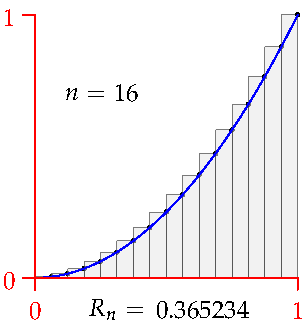
\includegraphics{area-up}\smallbreak
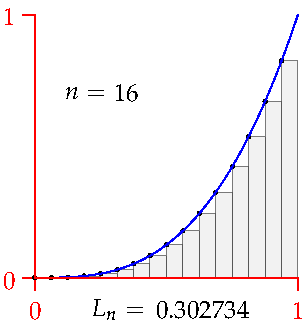
\includegraphics{area-down}}
\end{example}
\goodbreak

The example contains the essential idea, but more flexibility is needed. To get further, we must properly define the concepts of partition and Riemann sum.

\footnotetext{Now is a good time to review some identities:
	$\sum\limits_{i=1}^n i=\frac 12n(n+1)$, \ $\sum\limits_{i=1}^n i^2=\frac 16n(n+1)(2n+1)$, \ $\sum\limits_{i=1}^n i^3=\frac 14n^2(n+1)^2$}

\goodbreak

\begin{defn}{}{}
A \emph{partition} $P=\{x_0,\ldots,x_n\}$ of an interval $[a,b]$ is a finite sequence such that
\[a=x_0<x_1<\cdots< x_{n-1}< x_n=b\]
For each $1\le i\le n$, define $\Delta x_i=x_i-x_{i-1}$. The \emph{mesh} of the partition is $\mesh(P):=\max\Delta x_i$.\smallbreak
Choose a \emph{sample point} $x_i^*$ in each \emph{subinterval} $[x_{i-1},x_i]$.\smallbreak
If $f:[a,b]\to\R$, the \emph{Riemann sum} \smash{$\sum\limits_{i=1}^n f(x_i^*)\,\Delta x_i$} computes the area of a family of $n$ rectangles. 
\begin{center}
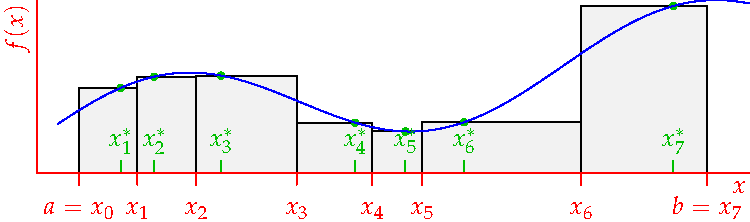
\includegraphics{riemann-sum}
\end{center}
\end{defn}

In elementary calculus, one typically computes Riemann sums for \emph{equally-spaced} partitions with \emph{left,} \emph{right} or \emph{middle} sample points. The double freedom of partition \& sample points makes applying the definition a challenge, so instead we consider two special families of rectangles. 


\begin{defn}{}{darbouxint}
Given a partition $P$ of $[a,b]$ and a bounded function $f$ on $[a,b]$, define\par
\begin{minipage}[t]{0.6\linewidth}\vspace{-15pt}
\begin{align*}
&M_i=\!\!\sup_{x\in [x_{i-1},x_i]}\! f(x)\qquad &&U(f,P)=\sum_{i=1}^n M_i\,\Delta x_i\\
&m_i=\!\!\inf_{x\in [x_{i-1},x_i]}\! f(x) &&L(f,P)=\sum_{i=1}^n m_i\,\Delta x_i
\end{align*}
$U(f,P)$ and $L(f,P)$ are the \emph{upper} and \emph{lower Darboux sums} for $f$ with respect to $P$.
The \emph{upper} and \emph{lower Darboux integrals} are
% \begin{gather*}
% U(f)=\upint_a^b f(x)\,\dx:=\inf\{U(f,P):P\text{ is a partition of $[a,b]$}\}\\
% L(f)=\lowint_a^bf(x)\,\dx:=\sup\{L(f,P):P\text{ is a partition of $[a,b]$}\}
% \end{gather*}
\[U(f)=\inf U(f,P)\qquad L(f)=\sup L(f,P)\]
where the supremum and infimum are over all partitions.\smallbreak
We say that $f$ is \emph{(Riemann) integrable}  on $[a,b]$ if $U(f)=L(f)$ and denote this value by
\[\int_a^bf\quad\text{or}\quad\int_a^bf(x)\,\dx\]
If the interval is understood or irrelevant, it is common just to say that $f$ is integrable and write $\int f$.
\end{minipage}\begin{minipage}[t]{0.4\linewidth}\vspace{0pt}
\centering
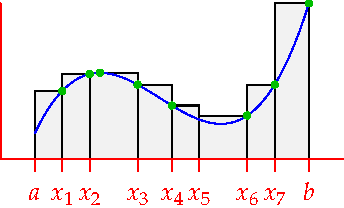
\includegraphics{riemann-sum-upper}\par
Upper Darboux sum $U(f,P)$\bigbreak
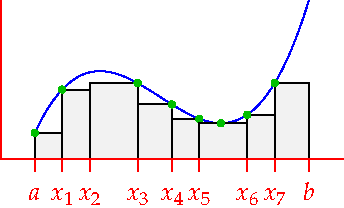
\includegraphics{riemann-sum-lower}\par
Lower Darboux sum $L(f,P)$
\end{minipage}
% We say that $f$ is integrable on a bounded interval $(a,b)$ if every extension of $f$ to $[a,b]$ is integrable.\smallbreak
\end{defn}


Intuitively, $L(f,P)$ is the sum of the areas of rectangles built on $P$ which just fit under the graph of $f$. It is also the infimum of all Riemann sums on $P$. If $f$ is discontinuous, then $L(f,P)$ need not be a Riemann sum; there might not be suitable sample points!

\goodbreak

\begin{examples}{}{}
\exstart We revisit Example \ref{ex:riemannintro} in this language.
\begin{enumerate}\setcounter{enumi}{1}
  \item[]Given a partition $Q=\{x_0,\ldots,x_n\}$ of $[0,1]$ and sample points $x_i^*\in[x_{i-1},x_i]$, we compute the Riemann sum for $f(x)=x^2$
	\[\sum_{i=1}^nf(x_i^*)\,\Delta x_i=\sum_{i=1}^n(x_i^*)^2(x_i-x_{i-1})\]
	Since $f$ is increasing,  we have $x_{i-1}^2\le (x_i^*)^2\le x_i^2$ on each interval, whence
	\[L(f,Q)=\sum_{i=1}^n(x_{i-1})^2(x_i-x_{i-1})
		\le \sum_{i=1}^n(x_i^*)^2(x_i-x_{i-1})
		\le\sum_{i=1}^n(x_i)^2(x_i-x_{i-1})=U(f,Q)\]
	The Darboux sums are therefore the Riemann sums for right and left endpoints.\smallbreak
	If we take $Q_n$ to be the partition with subintervals of equal width $\Delta x=\frac 1n$, then
	\[U(f)=\inf_P U(f,P)\le U(f,Q_n)=\sum_{i=1}^n\left(\frac in\right)^2\!\Delta x=R_n\]
	is the right Riemann sum discussed originally. Similarly $L(f)\ge L_n$. Since $L_n$ and $R_n$ both converge to $\frac 13$ as $n\to \infty$, the squeeze theorem forces
	\[L_n\le L(f)\le U(f)\le R_n\implies L(f)=U(f)=\frac 13\]
	whence $f$ is Riemann integrable on $[0,1]$ with $\int_0^1x^2\,\dx=\frac 13$.

\begin{minipage}[t]{0.55\linewidth}\vspace{0pt}
\item Suppose $f(x)=kx+c$ on the interval $[a,b]$ where $k>0$. Take the evenly spaced partition $P_n$ where $x_i=a+\frac{b-a}ni$ with $\Delta x_i=\frac{b-a}n$. Since $f$ is increasing, the upper Darboux sum is again the Riemann sum with right-endpoints:
	\begin{align*}
	U(f,P_n)&=R_n=\sum_{i=1}^nf(x_i)\Delta x\\
	&=\frac{b-a}n\sum_{i=1}^n\frac{k(b-a)}ni+ak+c
	\end{align*}
\end{minipage}\begin{minipage}[t]{0.45\linewidth}\vspace{0pt}
\flushright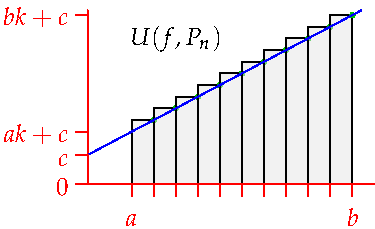
\includegraphics{darboux-triangle}
\end{minipage}\vspace{-5pt}
  
	\begin{align*}
	\phantom{U(f,P_n)}&=\frac{b-a}n\left[\frac{k(b-a)}n\cdot \frac 12n(n+1)+(ak+c)n\right]\\
	&\xrightarrow[n\to\infty]{} \frac 12k(b-a)^2+(b-a)(ak+c)=\frac k2(b^2-a^2)+c(b-a)
	\end{align*}
	We similarly see that the lower Darboux sum is given by the Riemann sum with left endpoints, and that 
	\[L(f,P_n)=L_n= \frac{b-a}n\left[\frac{k(b-a)}n\cdot \frac 12n(n-1)+(ak+c)n\right] \xrightarrow[n\to\infty]{} \frac k2(b^2-a^2)+c(b-a)
	\]
	By the same argument as above, $L_n\le L(f)\le U(f)\le R_n$ and the squeeze theorem show that $f$ is integrable with $\int_a^bf=\frac k2(b^2-a^2)+c(b-a)$. 
\end{enumerate}
\end{examples}

\goodbreak


\phantomsection\label{pg:riemanndefthm}
Following the examples, a few remarks are in order.
\begin{description}
  \item[\normalfont\emph{Riemann versus Darboux} ] Definition \ref{defn:darbouxint} is really that of the \emph{Darboux integral.} Riemann's definition is as follows: for $f[a,b]\to\R$ to be integrable with integral $\int_a^bf$ means
	\begin{gather*}
	\forall\epsilon>0,\ \exists\delta\text{ such that }\forall P,x_i^*,\ \mesh(P)<\delta\implies \nm{\sum\limits_{i=1}^nf(x_i^*)\Delta x_i-\int_a^bf}<\epsilon
	\end{gather*}
	It can be shown that this is equivalent to the Darboux integral. We won't pursue Riemann's formulation further, except to observe that \emph{if} a function is integrable and $\mesh(P_n)\to 0$, then $\int_a^b f=\lim\limits_{n\to\infty}\sum\limits_{i=1}^nf(x_i^*)\Delta x_i$: this allows us to approximate integrals using any sample points we choose, hence why \emph{right} endpoints ($x_i^*=x_i$) are so common in Freshman calculus.
  \item[\normalfont\emph{Monotone Functions} ] Darboux sums are particularly easy to compute for monotone functions. As in the examples, if $f$ is increasing, then each $M_i=f(x_i)$, from which $U(f,P)$ is the Riemann sum with \emph{right-endpoints.} Similarly, $L(f,P)$ is the Riemann sum with \emph{left-endpoints.} The roles reverse if $f$ is decreasing.
  \item[\normalfont\emph{Area} ] If $f$ is positive and continuous,\footnote{We'll see later (Theorem \ref{thm:monotoneint}) that every continuous function is integrable.} the Riemann integral $\int_a^bf$ serves as a \emph{definition} for the area under the curve $y=f(x)$. This should make intuitive sense:
  \begin{enumerate}
    \item In the second example where we have a straight line, we obtain the same value for the area by computing directly as the sum of a rectangle and a triangle!
    \item If the area under the curve is to make sense, then, for any partition $P$, it plainly satisfies the inequalities
  	\[L(f,P)\le \text{Area}\le U(f,P)\]
  	But these are exactly the same as those satisfied by the integral itself:
  	\[L(f,P)\le L(f)=\int_a^bf=U(f)\le U(f,P)\]
  \end{enumerate}
\end{description}


In the examples we exhibited a sequence of partitions $(P_n)$ where $U(f,P_n)$ and $L(f,P_n)$ both converged to the same limit. The next results develop some basic properties of partitions and make this process rigorous.


\begin{lemm}{}{partitionseqlemm}
Suppose $f:[a,b]\to\R$ is bounded and suppose $P,Q$ are partitions of $[a,b]$.
\begin{enumerate}
  \item If $Q$ is a \emph{refinement} of $P$, that is $P\subseteq Q$, then
  \[L(f,P)\le L(f,Q)\le U(f,Q)\le U(f,P)\]
  \item For any partitions $P,Q$, we have $L(f,P)\le U(f,Q)$
  \item $L(f)\le U(f)$
\end{enumerate} 
\end{lemm}

\goodbreak

\begin{proof}
\exstart We prove inductively. First suppose that $Q=P\cup\{t\}$ contains exactly one additional point $t\in(x_{k-1},x_k)$. Write\par
\begin{minipage}[t]{0.6\linewidth}\vspace{-15pt}
\begin{enumerate}
  \item[]\begin{gather*}
  m_1=\inf\{f(x):x\in[x_{k-1},t]\}\\
  m_2=\inf\{f(x):x\in[t,x_{k-1}]\}\\
  m=\inf\{f(x):x\in[x_{k-1},x_k]\}=\min\{m_1,m_2\}\\[-15pt]
  \end{gather*}
  The Darboux sums $L(f,P)$ and $L(f,Q)$ are identical except for the terms involving $t$; indeed
  \end{enumerate}
\end{minipage}\begin{minipage}[t]{0.4\linewidth}\vspace{-17pt}
\flushright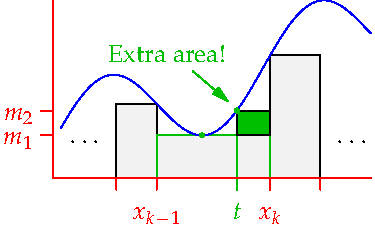
\includegraphics{riemann-sum3}
\end{minipage}\par\vspace{-17pt}
\begin{enumerate}\setcounter{enumi}{1}
  \item[]\begin{align*}
  L(f,Q)-L(f,P) &=m_1(t-x_{k-1}) +m_2(x_{k}-t) -m(x_k-x_{k-1})\\
  &=(m_1-m)(t-x_{k-1}) +(m_2-m)(x_k-t)\ge 0
  \end{align*}
  Since partitions are finite sets, by induction we see that $P\subseteq Q\implies L(f,P)\le L(f,Q)$.\smallbreak
  The argument for $U(f,Q)\le U(f,P)$ is similar, and the middle inequality is trivial.
  
  \item If $P$ and $Q$ are partitions, then $P\cup Q$ is a refinement of both $P$ and $Q$. By part 1,
  \[L(f,P)\le L(f,P\cup Q)\le U(f,P\cup Q)\le U(f,Q)\tag{$\ast$}\]
  
	\item We leave this as an exercise.\qedhere
\end{enumerate}
\end{proof}

\begin{thm}{Cauchy criterion for integrability}{partitionseq}
Suppose $f:[a,b]\to\R$ is bounded.
\begin{enumerate}
  \item $f$ is integrable $\iff\forall\epsilon>0$, $\exists P$ such that $U(f,P)-L(f,P)<\epsilon$
  \item $f$ is integrable $\iff\exists (P_n)_{n\in\N}$ such that $U(f,P_n)-L(f,P_n)\to 0$. Moreover, in such a case both sequences $U(f,P_n)$ and $L(f,P_n)$ converge to $\int_a^bf$.
\end{enumerate} 
\end{thm}

We call this a Cauchy criterion since integrability is demonstrated without mention of the integral! 


\begin{proof}
\begin{enumerate}
	\item ($\Rightarrow$)\quad Suppose $f$ is integrable. Since $\inf U(f,Q)=\int f=\sup L(f,R)$, $\exists Q,R$ such that
	\[U(f,Q)-\int f<\frac\epsilon 2\quad\text{and}\quad \int f-L(f,R)<\frac \epsilon 2\]
	Let $P=Q\cup R$ and apply ($\ast$): \ $L(f,R)\le L(f,P)\le U(f,P)\le U(f,Q)$. But then
	\[U(f,P)-L(f,P)\le U(f,Q)-L(f,R) =U(f,Q)-\int f+\int f-L(f,R)<\epsilon\]
	($\Leftarrow$)\quad For every partition, $L(f,P)\le L(f)\le U(f)\le U(f,P)$. Thus
	\[0\le U(f)-L(f)\le U(f,P)-L(f,P)<\epsilon\]
	Since this holds for all $\epsilon>0$, we see that $U(f)=L(f)$.
	\item This is an exercise.\qedhere
\end{enumerate}
\end{proof}

\goodbreak


\begin{examples}{}{riemannint2}
\exstart The freedom to choose a partition can be very useful. Consider $f(x)=\sqrt x$ on the interval $[0,b]$. We choose a partition that evaluates nicely when fed to this function:
  \begin{gather*}
  P_n=\{x_0,\ldots,x_n\}\quad\text{where}\quad x_i=\left(\frac in\right)^2b\\
  \implies \Delta x_i=x_i-x_{i-1}=\frac b{n^2}\bigl(i^2-(i-1)^2\bigr)=\frac{(2i-1)b}{n^2}
  \end{gather*}
  Since $f$ is increasing on $[0,b]$, we see that
  \begin{align*}
  U(f,P_n)&=\sum_{i=1}^nf(x_i)\Delta x_i =\sum_{i=1}^n\frac{i\sqrt b}n\cdot\frac{(2i-1)b}{n^2} =\frac{b^{3/2}}{n^3}\sum_{i=1}^n2i^2-i \\
  &=\frac{b^{3/2}}{n^3}\left[\frac 13n(n+1)(2n+1)-\frac 12n(n+1)\right] \xrightarrow[n\to\infty]{}\frac 23b^{3/2}
  \end{align*}
  Similarly
  \begin{align*}
  L(f,P_n)&=\sum_{i=1}^nf(x_{i-1})\Delta x_i =\sum_{i=1}^n\frac{(i-1)\sqrt b}n\cdot\frac{(2i-1)b}{n^2} =\frac{b^{3/2}}{n^3}\sum_{i=1}^n2i^2-3i+1 \\
  &=\frac{b^{3/2}}{n^3}\left[\frac 13n(n+1)(2n+1)-\frac 32n(n+1) +n\right] \xrightarrow[n\to\infty]{}\frac 23b^{3/2}
  \end{align*}
  Since these limits are equal, we conclude that $f$ is integrable and that $\int_0^b\sqrt x\,\dx=\frac 23b^{3/2}$.

\begin{enumerate}\setcounter{enumi}{1}
  \item[]\begin{center}
  \begin{tabular}{c@{\qquad}c}
  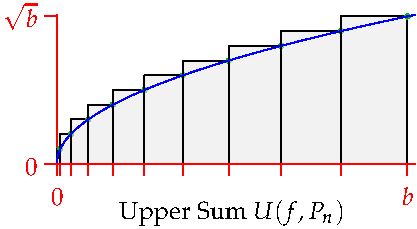
\includegraphics{darboux-ex1}
  &
  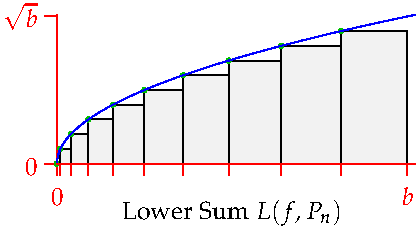
\includegraphics{darboux-ex2}
  \end{tabular}
  \end{center}
  
	\item We finish this section with the classic example of a non-integrable function. Let $f:[a,b]\to\R$ to be the indicator function of the irrational numbers,
	\[f(x)=\begin{cases}
	1&\text{if }x\not\in\Q\\
	0&\text{if }x\in\Q
	\end{cases}\]
	Since any interval of positive length contains both rational and irrational numbers, we see that
	\[\sup\bigl\{f(x):x\in[x_{i-1},x_i]\bigr\}=1\quad\text{and}\quad \inf\bigl\{f(x):x\in[x_{i-1},x_i]\bigr\}=0\]
	for \emph{any} partition $P=\{x_0,\ldots,x_n\}$. We conclude that
	\begin{gather*}
	U(f,P)=\sum_{i=1}^n(x_i-x_{i-1})=b-a\implies U(f)=b-a\quad\text{and}\\
	L(f,P)=0\implies L(f)=0
	\end{gather*}
	Since the upper and lower integrals are unequal, $f$ is not Riemann integrable.
\end{enumerate}
\end{examples}


% \begin{asidep}
% The definition we have given is strictly that of the \emph{Darboux integral}. Riemann's definition is as follows:
% 
% \begin{defn}
% Let $f$ be bounded on $[a,b]$ and let $P$ be a partition. A \emph{Riemann sum} of $f$ associated to $P$ is a sum
% \[\sum_{k=1}^nf(x_k)(t_k-t_{k-1}),\text{ where }x_k\in[t_{k-1},t_k].\]
% $f$ is \emph{Riemann integrable} on $[a,b]$ with integral $r$ if for all $\epsilon>0$ there exists $\delta>0$ such that for all Riemann sums $S$ with partitions finer than $\delta$ (i.e. $t_k-t_{k-1}<\delta$ for all $k$) we have
% \[\nm{S-r}<\epsilon.\]
% \end{defn}
% 
% It is common to use the term Riemann integral for either Riemann's or Darboux's definition since they coincide (by contrast, alternative definitions of the integral allow more functions to be considered integrable). Indeed we have the following theorem:
% 
% \begin{thm}
% $f$ is Riemann integrable on $[a,b]$ iff it is Darboux integrable on $[a,b]$, in which case the values of the integrals coincide.
% \end{thm}
% 
% In order to prove the theorem, and several others in the next section, it is convenient to have the following definition and $\epsilon$--$\delta$ criterion for integrability, which we state without its uninstructive proof.
% 
% \begin{defn}
% Given a partition $P=\{t_0<\cdots<t_n\}$ of $[a,b]$, the \emph{mesh} of $P$ is the maximum of the distances between successive $t_k$. I.e. $\mesh(P)=\max(t_k-t_{k-1})$.
% \end{defn}
% 
% \begin{prop}\label{prop:intepsilon}
% A bounded function $f$ on $[a,b]$ is integrable iff either of the following conditions hold:
% \begin{enumerate}
%   \item For each $\epsilon>0$ there exists a partition $P$ of $[a,b]$ such that
% \[U(f,P)-L(f,P)<\epsilon.\]
% \item For all $\epsilon>0$ there exists $\delta>0$ such that
% \[\mesh(P)<\delta\Longrightarrow U(f,P)-L(f,P)<\epsilon.\]
% \end{enumerate}
% \end{prop}
% 
% The proposition is intuitive in the sense that we visualize the upper and lower Darboux sums as converging to the integral. This is, of course, not technically correct, since there is no sequence of Darboux sums.
% 
% \begin{proof}[Proof of Theorem]
% Suppose $f$ is Darboux integrable and let $\epsilon>0$ be chosen. Let $\delta>0$ be chosen satisfying Proposition \ref{prop:intepsilon}. Let $P$ be any partition of $[a,b]$ with $\mesh(P)<\delta$ and let $S$ be a Riemann sum associated to $P$. Clearly we have
% \[L(f,P)\le S\le U(f,P).\]
% By Proposition \ref{prop:intepsilon} we have
% \[U(f,P)<L(f,P)+\epsilon\le L(f)+\epsilon.\]
% Similarly
% \[L(f,P)>U(f,P)-\epsilon\ge U(f)-\epsilon.\]
% Since $U(f)=L(f)=\int_a^bf$ we see that
% \[\int_a^bf-\epsilon<S<\int_a^b+\epsilon.\]
% Hence $f$ is Riemann integrable, with integral $r=\int_a^bf$.\\
% Now suppose $f$ is Riemann integrable with integral $r$. Let $\epsilon>0$ be given, $\delta>0$ satisfying the definition and $P$ a partition finer than $\delta$. Then any Riemann sum associated to $P$ satisfies
% \[\nm{S-r}<\epsilon.\]
% Since $\epsilon>0$ we may select $x_k\in[t_{k-1},t_k]$ such that
% \[f(x_k)>\sup\{f(x):x\in[t_{k-1},t_k]\}-\epsilon.\]
% The Riemann sum $S$ for these $x_i$ clearly satisfies
% \[S\ge U(f,P)-\epsilon(b-a).\]
% But then, for all $\epsilon>0$ we have
% \[U(f)\le U(f,P)\le S+\epsilon(b-a)\le r+\epsilon+\epsilon(b-a)=r+\epsilon(1+b-a),\]
% so that $U(f)\le r$. Similarly we see that $L(f)\ge r$. Then $U(f)\ge L(f)$ implies equality and so $f$ is Darboux integrable with integral $\int_a^bf=r$.
% \end{proof}
% \end{asidep}\newpage

As any freshman calculus student can attest, if you can find an anti-derivative, then the fundamental theorem of calculus (Section \ref{sec:ftc}) makes evaluating integrals far easier. For instance, you are probably desperate to write
\[\diff x\frac 23x^{3/2}=x^{1/2}\implies\int_0^b\sqrt x\,\dx=\frac 23x^{3/2}\Big|_0^b=\frac 23b^{3/2}\]
rather than computing Riemann/Darboux sums as in the previous example! In most practical cases, however, no easy-to-compute anti-derivative exists, so the best we can do is approximate integrals by evaluating Riemann sums for progressively finer partitions. Thankfully computers excel at such tedious work!

\begin{exercises}
\exstart For each function on the given interval, use partitions to find the upper and lower Darboux integrals. Hence prove that the function is integrable and compute its integral.
\begin{enumerate}\setcounter{enumi}{1}
	\item[]\begin{enumerate}
	  \item $f(x)=x^3$ on $[0,b]$ for any $b>0$.
	  
	  \item $g(x)=\sqrt[3]{x}$ on $[0,b]$.\smallbreak
	  (\emph{Hint: mimic Example \hyperref[ex:riemannint2]{\ref*{ex:riemannint2}.1})}
	\end{enumerate}
	
	\item Repeat question 1 for the following two functions. You \emph{cannot} simply compute Riemann sums for left and right endpoints and take limits: why not?
	\begin{enumerate}  
	  \item $h(x)=x(2-x)$ on $[0,2]$\smallbreak
	  (\emph{Hint: choose a partition with $2n$ points such that $x_n=1$ and observe that $h(2-x)=h(x)$})
	  
	  \item $k(x)=\begin{cases}
	  2x&\text{if }x\le 1\\
	 	5-x&\text{if }x>1
	  \end{cases}$ on $[0,3]$.\smallbreak
	  (\emph{Hint: this time try a partition with $3n$ points\ldots})
	\end{enumerate}

  \item Let $f(x)=x$ for rational $x$ and $f(x)=0$ for irrational $x$.
    \begin{enumerate}
    \item Calculate the upper and lower Darboux integrals for $f$ on the interval $[0,b]$.
    \item Is $f$ integrable on $[0,b]$?
    \end{enumerate}
    
	\item Prove part 3 of Lemma \ref{lemm:partitionseqlemm}: $L(f)\le U(f)$.

	\item Prove part 2 of Theorem \ref{thm:partitionseq}.
 	\begin{quote}
 	$f$ is integrable $\iff\exists (P_n)_{n\in\N}$ such that $U(f,P_n)-L(f,P_n)\to 0$.
 	\end{quote}
 	Moreover, both $U(f,P_n)$ and $L(f,P_n)$ converge to $\int f$.
	
	\item\begin{enumerate}
	  \item Reread Definition \ref{defn:darbouxint}. What happens if we allow $f:[a,b]\to\R$ to be \emph{unbounded}?
	  \item Read ``\emph{Riemann versus Darboux}'' on page \pageref{pg:riemanndefthm}. Explain why being \emph{Riemann} integrable also forces $f$ to be bounded.
	\end{enumerate}

	\item (If you like coding)\quad Write a short program to estimate $\int_a^bf(x)\,\dx$ using Riemann sums. This can be very simple (equal partitions with right endpoints), or more complex (random partition and sample points given a mesh). Apply your program to estimate $\int_0^{5}\sin(x^2e^{-\sqrt x})\,\dx$.
\end{enumerate}
\end{exercises}


\clearpage


\subsection{Properties of the Riemann Integral}\label{sec:riemannproperties}

The rough take-away of this long section is that everything you think is integrable probably is! There will not be many examples since we have not established many explicit values for integrals.


\begin{thm}{Linearity}{intlinear}
If $f,g$ are integrable and $k,l$ are constant, then $kf+lg$ is integrable and
\[\int  kf+lg=k\int f+l\int g\]
\end{thm}

\begin{example}{}{}
Thanks to examples in the previous section, we can now calculate, for instance
\[\int_0^25x^3-3\sqrt x\,\dx=5\cdot\frac 14\cdot 2^4 -3\cdot \frac 23\cdot 2^{3/2} =20-4\sqrt 2\]
\end{example}

\begin{proof}
	Suppose $\epsilon>0$ is given. By Theorem \ref{thm:partitionseq} part 3, there exist partitions $R,S$ such that
	\[U(f,R)-L(f,R)<\smash{\frac\epsilon 2}\quad\text{and}\quad U(g,S)-L(g,S)<\smash{\frac\epsilon 2}\]
	By Theorem \ref{thm:partitionseq} part 1, if $P:=R\cup S$, then both inequalities are satisfied by $P$. On each subinterval,
	\[\inf f(x)+\inf g(x)\le \inf(f(x)+g(x))\quad\text{and}\quad \sup(f(x)+g(x))\le\sup f(x)+\sup g(x)\]
	since the individual suprema/infima could be `evaluated' at different places. Thus
	\[L(f,P)+L(g,P)\le L(f+g,P)\le U(f+g,P)\le U(f,P)+U(g,P)\]
	whence $U(f+g,P)-L(f+g,P)<\epsilon$ and $f+g$ is integrable. Moreover,
	\begin{gather*}
	\int(f+g)-\int f-\int g \le \Bigl(U(f,P)-\int f\Bigr)+\Bigl(U(g,P)-\int g\Bigr)<\epsilon
	\end{gather*}
	Using lower Darboux integrals similarly, we see that
	\[-\epsilon<\int(f+g)-\int f-\int g<\epsilon\]
	Since this holds for all $\epsilon>0$, we conclude that $\int(f+g)=\int f+\int g$.\smallbreak
	That $kf$ is integrable with $\int kf=k\int f$ is an exercise. Put these together for the result.
\end{proof}

\begin{cor}{Changing endvalues}{intopen}
Suppose $g$ is integrable on $[a,b]$ and that $f:[a,b]\to\R$ satisfies $f(x)=g(x)$ on $(a,b)$. Then $f$ is integrable on $[a,b]$ and $\int_a^b f=\int_a^b g$.
\end{cor}

\begin{defn}{Integration on an open interval}{intopen}
A \emph{bounded} function $f:(a,b)\to\R$ is \emph{integrable} if it has an integrable extension $g:[a,b]\to\R$ where $f(x)=g(x)$ on $(a,b)$.
In such a case, we define $\int_a^bf:=\int_a^bg$.
\end{defn}

The Corollary (its proof is an exercise) shows that the choice of extension is irrelevant.


\goodbreak


\begin{thm}{Basic Comparisons}{intineq}
Suppose $f$ and $g$ are integrable on $[a,b]$.
\begin{enumerate}\itemsep1pt\parsep=1pt
  \item If $f(x)\le g(x)$, then $\int f\le\int g$.
  \item If $m\le f(x)\le M$ then $m(b-a)\le\int_a^bf\le M(b-a)$.
  \item $fg$ is integrable.
  \item $\nm f$ is integrable and $\nm{\int f}\le\int \nm f$.
  \item $\max(f,g)$ and $\min(f,g)$ are integrable.
\end{enumerate}
\end{thm}

Part 3 is \emph{not} integration by parts and does \emph{not} tell us how $\int fg$ relates to $\int f$ and $\int g$!

\begin{proof}
\begin{enumerate}\itemsep=1pt\parsep=1pt
  \item Since $g(x)-f(x)\ge 0$ is integrable, $L(g-f,P)\ge 0$ for all partitions $P$, and so
  \[\smash{0\le L(g-f)=\int g-f=\int g-\int f}\]
  \item Apply part 1 twice.
  \item This is an exercise.
  \item The integrability is an exercise. For the comparison, apply part 1 to $-\nm f\le f\le\nm f$.
  \item $\max(f,g)=\frac 12(f+g)+\frac 12\nm{f-g}$, etc.\hfill\qedhere
\end{enumerate}
\end{proof}





\begin{thm}[lower separated=false, sidebyside, sidebyside align=top seam, sidebyside gap=0pt, righthand width=0.35\linewidth]{Domain splitting}{domainsplit}
Suppose that $f:[a,b]\to\R$ and let $c\in(a,b)$. If $f$ is integrable on both $[a,c]$ and $[c,b]$, then it is integrable on $[a,b]$ and
\[\int_a^bf=\int_a^cf+\int_c^bf\]
\tcblower
\flushright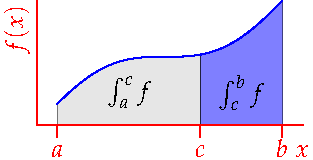
\includegraphics{domain-split}
\end{thm}

In light of this result, it is conventional to allow integral limits to be reversed:
\[\int_b^af:=-\int_a^bf\quad\text{ is consistent with }\quad \int_a^af=0\]


\begin{proof}
Let $\epsilon>0$ be given, then $\exists R,S$ partitions of $[a,c],[c,b]$ such that\par
\begin{minipage}[t]{0.65\linewidth}\vspace{-10pt}
\[U(f,R)-L(f,R)<\frac\epsilon 2,\qquad U(f,S)-L(f,S)<\frac\epsilon 2\]
Choose $P=R\cup S$ to partition $[a,b]$, then
\[U(f,P)-L(f,P)=U(f,R)+U(f,S)-L(f,R)-L(f,S)<\epsilon\]
Moreover
\end{minipage}\begin{minipage}[t]{0.35\linewidth}\vspace{0pt}
\flushright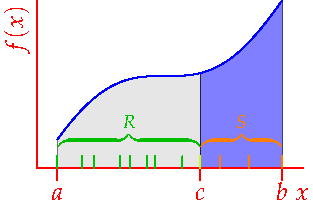
\includegraphics{domain-split2}
\end{minipage}\par
\[\int_a^bf-\int_a^cf-\int_c^bf\le U(f,P)-L(f,R)-L(f,S)=U(f,P)-L(f,P)<\epsilon\]
The other side is similar.
\end{proof}

\goodbreak

\begin{example}{}{}
If $f(x)=\sqrt x$ on $[0,1]$ and $f(x)=1$ on $[1,2]$, then
\[\int_0^2f=\int_0^1\sqrt x\,\dx+\int_1^2 1\,\dx=\frac 23+1=\frac 53\]
\end{example}


\boldsubsubsection{Monotonic \& Continuous Functions}

We are now in a position to establish the integrability of two large classes of functions.

\begin{defn}{}{}
A function $f:[a,b]\to\R$ is:
\begin{description}\itemsep3pt\parsep3pt
	\item[\normalfont\emph{Monotonic}] if it is either \emph{increasing} ($x<y\implies f(x)\le f(y)$) or \emph{decreasing}.
	\item[\normalfont\emph{Piecewise monotonic}] if there is a partition $P=\{x_0,\ldots,x_n\}$ of $[a,b]$ such that $f$ is monotonic on each open subinterval $(x_{k-1},x_k)$.
	\item[\normalfont\emph{Piecewise continuous}] if there is a partition such that $f$ is \emph{uniformly} continuous on each $(x_{k-1},x_k)$.
\end{description}
\end{defn}

\begin{thm}{}{monotoneint}
If $f$ is \emph{monotonic} or \emph{continuous} on $[a,b]$, then it is integrable.
\end{thm}

%Note again that we do not obtain explicit \emph{formulæ.}


% \begin{thm}{Continuous Functions}{intcont}
% Every continuous function $f$ on $[a,b]$ is integrable.
% \end{thm}



\begin{examples}{}{}
\exstart Since sine is continuous, we can approximate via a sequence of Riemann sums
\[\int_0^\pi\sin x\,\dx =\frac\pi{n}\lim_{n\to\infty}\sum_{i=1}^n\sin\frac{\pi i}{n}\]
\emph{Evaluating} this limit is another matter entirely, one best handled in the \hyperref[sec:ftc]{next section}...
\begin{enumerate}\setcounter{enumi}{1}
  \item Similarly, $e^{\sqrt x}$ can be integrated and therefore approximated via Riemann sums:
  \[\displaystyle\int_0^1 e^{\sqrt x}\,\dx =\frac 1{n}\lim\limits_{n\to\infty}\sum_{i=1}^n \exp\sqrt{\frac in} = \lim\limits_{n\to\infty}\sum_{i=1}^n \frac{2j-1}n\exp\frac jn\]
  Both sums use right endpoints; the first has equal subintervals and the second is analogous to Example \hyperref[ex:riemannint2]{\ref*{ex:riemannint2}.1}. These limits would typically be estimated using a computer.
\end{enumerate}
\end{examples}

\begin{proof}
Suppose $f:[a,b]\to\R$ is continuous. Since $[a,b]$ is closed and bounded, $f$ is \emph{uniformly} continuous. Let $\epsilon>0$ be given:
\[\exists\delta>0\text{ such that }\forall x,y\in[a,b],\ \nm{x-y}<\delta\implies\nm{f(x)-f(y)}<\frac\epsilon{b-a}\]
Let $P$ be a partition with $\mesh P<\delta$. Since $f$ attains its bounds on each $[x_{i-1},x_i]$ (extreme value theorem),
\[
\exists x_i^*,y_i^*\in [x_{i-1},x_i]\quad\text{such that}\quad M_i-m_i=f(x_i^*)-f(y_i^*)<\frac\epsilon{b-a}
\]
from which
\[
U(f,P)-L(f,P)<\smash[t]{\sum_{i=1}^n}\frac\epsilon{b-a}(x_i-x_{i-1})=\epsilon
\]
The monotonicity argument is an exercise.
\end{proof}

\goodbreak

\begin{cor}{}{piecewiseint}
Piecewise continuous and \emph{bounded} piecewise monotonic functions are integrable.
\end{cor}

\begin{proof}
If $f$ is piecewise continuous, then the restriction of $f$ to $(x_{k-1},x_k)$ has a continuous extension $g_k:[x_{k-1},x_k]\to\R$; integrable by Theorem \ref{thm:monotoneint}. By Corollary \ref{cor:intopen}, $f$ is integrable on $[x_{k-1},x_k]$ with $\int_{x_{k-1}}^{x_k}f=\int_{x_{k-1}}^{x_k}g_k$. Several applications of Theorem \ref{thm:domainsplit} finish things off:
\[\int_a^bf=\sum_{k=1}^n\int_{x_{k-1}}^{x_k}f\]
The argument for piecewise monotonicity is similar.
\end{proof}

\begin{example}[lower separated=false, sidebyside, sidebyside align=top seam, sidebyside gap=0pt, righthand width=0.35\linewidth]{}{fracpart}
The `fractional part' function $f(x)=x-\lfloor x\rfloor$ is both piecewise continuous and piecewise monotone on any bounded interval. It is therefore integrable on any $[a,b]$.
\tcblower
\flushright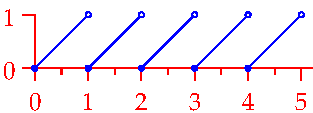
\includegraphics{fracpart}
\end{example}

\goodbreak

We finish with the final incarnation of the intermediate value theorem.

\begin{cor}{IVT for integrals}{}
If $f$ is continuous on $[a,b]$, then $\exists \xi\in (a,b)$ for which
\[f(\xi)=\frac 1{b-a}\int_a^bf\]
\end{cor}

\begin{proof}%\squeezeeqn{8pt}
Since $f$ is continuous, it is integrable on $[a,b]$. By the extreme value theorem it is also bounded and attains its bounds: $\exists p,q\in[a,b]$ such that\par
\begin{minipage}[t]{0.55\linewidth}\vspace{-5pt}
\[f(p):=\inf\limits_{x\in[a,b]}f(x),\qquad f(q)=\sup\limits_{x\in[a,b]}f(x)\]
Applying Theorem \ref{thm:intineq}, part 2, with $m=f(p)$ and $M=f(q)$, we see that
\[(b-a)f(p)\le\int_a^bf\le (b-a)f(q)\]
\end{minipage}\begin{minipage}[t]{0.45\linewidth}\vspace{-5pt}
\flushright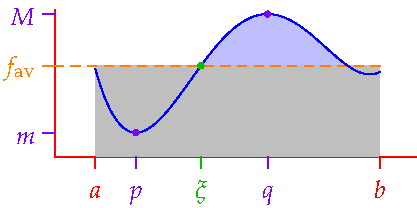
\includegraphics{average}
\end{minipage}\bigbreak

Now divide by $b-a$ and apply the usual intermediate value theorem for $f$ to see that the required $\xi$ exists between $p$ and $q$.
\end{proof}

In the picture, when $f$ is positive and continuous, the grey area equals that under the curve; imagine levelling off the blue hill with a bulldozer\ldots The notation $\textcolor{orange}{f_{\text{av}}}=\frac 1{b-a}\int_a^bf$ is short for the \textcolor{orange}{average value} of $f$ on $[a,b]$: to see why this interpretation is sensible, approach $\int f$ via a sequence of Riemann sums on equally-spaced partitions $P_n$, then
\[\frac 1{b-a}\int_a^b f =\lim_{n\to\infty}\sum_{i=1}^nf(x_i^*)\Delta x=\lim_{n\to\infty}\frac{f(x_1^*)+\cdots+f(x_n^*)}n\]
is the limit of a sequence of \emph{averages} of equally-spaced samples $f(x_i^*)$.

\goodbreak

\boldsubsubsection{What can/can't be integrated? (non-examinable)}

We now know a great many examples of integrable functions: essentially
\begin{itemize}\itemsep0pt
  \item Piecewise continuous \& monotonic functions are integrable.
  \item Linear combinations, products, absolute values, maximums and minimums of (already) integrable functions.
\end{itemize}

After so many positive integrability conditions, it is reasonable to ask precisely which functions are Riemann integrable. There is a precise answer, though it is quite tricky to understand.

\begin{thm}{Lebesgue}{}
Suppose $f:[a,b]\to\R$ is bounded. Then
\begin{quote}
$f$ is Riemann integrable $\iff$ it is continuous except on a set of \emph{measure zero}
\end{quote}
\end{thm}

Naïvely, the \emph{measure} of a set is the sum of the lengths of its maximal subintervals; though unfortunately this doesn't make for a very useful definition.\footnote{Formally, the \emph{length} of an open interval $(a,b)$ is $b-a$ and a set $A\subseteq \R$ has \emph{measure zero} if
\[\forall\epsilon>0,\ \exists \text{ open intervals $I_n$ such that }A\subseteq\bigcup_{n=1}^\infty I_n\text{ and }\sum_{i=1}^\infty\operatorname{length}(I_n)<\epsilon\]
More generally, the \emph{measure} of a set (subject to a technical condition) is the infimum of the sum of the lengths of any countable collection of open covering intervals. A rigorous discussion of \emph{measure theory} is properly a matter for graduate analysis. %To give you some idea of the difficulty, here is a more formal definition: the \emph{(Lebesgue) measure} of a set is the infimum of the sum of the lengths of any countable collection of open covering intervals
% \[
% \mu(A)=\inf\left\{\sum_{n=1}^\infty (b_n-a_n):A\subseteq\bigcup_{n=1}^\infty (a_n,b_n)\right\}
% \]
Somewhat surprisingly, there exist \href{https://en.wikipedia.org/wiki/Smith-Volterra-Cantor_set}{sets} with positive measure that contain no subintervals, and even sets which are non-measurable!} Any countable subset has measure zero; Lebesgue's result is almost as if we can extend Corollary \ref{cor:piecewiseint} to allow for infinite sums. Indeed you might have encountered a function which is continuous only on the irrationals; such a function is Riemann integrable. There are also some uncountable sets with measure zero such as Cantor's middle-third set: if $f$ is the indicator function of Cantor's set
\[f(x)=\begin{cases}
1&\text{if }x\in\mathcal C\\
0&\text{otherwise}
\end{cases}\]
then $f$ is continuous except on $\mathcal C$, and is Riemann integrable with $\int_0^1 f(x)\,\dx=0$.


\vfil

\begin{exercises}
\exstart Explain why $\int_{0}^{2\pi}x^2\sin^8(e^x)\,\dx \le\frac 83\pi^3$

\begin{enumerate}\setcounter{enumi}{1}
	\item If $f$ is integrable on $[a,b]$ prove that it is integrable on any interval $[c,d]\subseteq[a,b]$.
	
	\item We complete the proof of Theorem \ref{thm:intlinear} (linearity of integration).
	\begin{enumerate}
  	\item Suppose $k>0$, let $A\subseteq\R$ and define $kA:=\{kx:x\in A\}$. Prove that $\sup kA=k\sup A$ and $\inf kA=k\inf A$.
  	\item If $k>0$ prove that $kf$ is integrable on any interval and that $\int kf=k\int f$.
  	\item How should you modify your argument if $k<0$?
	\end{enumerate}
%  This is trivial if $k=0$. Assume $k>0$, then,\footnote{If $A$ is any set and $kA:=\{ka:a\in A\}$, then
% 	\[\sup(kA)=\begin{cases}
% 	k\sup A&\text{if $k>0$}\\
% 	k\inf A&\text{if $k<0$}
% 	\end{cases}
% 	\quad\text{and}\quad
% 	\inf(kA)=\begin{cases}
% 	k\inf A&\text{if $k>0$}\\
% 	k\sup A&\text{if $k<0$}
% 	\end{cases}\]}
% 	\[U(kf,P)=kU(f,P)\implies U(kf)=kU(f)\]
% 	Similarly $L(kf)=kL(f)$, from which $L(kf)=U(kf)=k\int f$.\\[5pt]
% 	If $k<0$, we instead observe that $L(kf)=kU(f)$, etc., for the same result.
	
  
  \item Give an example of an integrable but \emph{discontinuous} function on a closed bounded interval $[a,b]$ for which the conclusion of the Intermediate Value Theorem for Integrals is \emph{false.}
  
	\item Explicitly compute the value of the integral $\int_{1/2}^{{15/2}} x-\lfloor x\rfloor \,\dx$ (recall Example \ref{ex:fracpart}).
	
	\item\label{exs:extensionlemma} We prove and extend Corollary \ref{cor:intopen}. Suppose $f$ is integrable on $[a,b]$. 
	\begin{enumerate}
	  \item If $g:[a,b]\to\R$ satisfies $f(x)=g(x)$ for all $x\in (a,b)$, prove that $g$ is integrable and $\int_a^bg=\int_a^bf$.\smallbreak
		(\emph{Hint: consider $h=f-g$ and show that $\int h=0$})
		\item Now suppose $g:[a,b]\to\R$ satisfies $f(x)=g(x)$ for all $x\in [a,b]$ except at finitely many points. Prove that $g$ is integrable and $\int_a^bg=\int_a^bf$.
	\end{enumerate}
  
  \item Show that an increasing function on $[a,b]$ is integrable and thus complete Theorem \ref{thm:monotoneint}.\smallbreak
  (\emph{Hint: Choose a partition $P$ with $\mesh P<\frac\epsilon{f(b)-f(a)}$})
 
  
  \item Suppose $f$ and $g$ are integrable on $[a,b]$.
	\begin{enumerate}
    \item Define $h(x)=(f(x))^2$. We know:
  	\begin{itemize}
    	\item $f$ is bounded: $\exists K$ such that $\nm{f(x)}\le K$ on $[a,b]$.
    	\item Given $\epsilon>0$, $\exists P$ such that $U(f,P)-L(f,P)<\frac\epsilon{2K}$.
  		For each subinterval $[x_{i-1},x_i]$, let
  		\[M_i=\sup f(x),\qquad m_i=\inf f(x),\qquad \cl M_i=\sup h(x),\qquad \cl m_i=\inf h(x)\]
  	\end{itemize}
  	Prove that $\cl M_i-\cl m_i\le 2(M_i-m_i)K$ and use this to conclude that $h$ is integrable.
  	\item Prove that $fg$ is integrable.\smallbreak
  	(\emph{Hint: $fg=\frac 14(f+g)^2-\frac 14(f-g)^2$})
  	\item Prove that $U(\nm f,P)-L(\nm f,P)\le U(f,P)-L(f,P)$ for any partition $P$. Hence conclude that $\nm f$ is integrable.
  \end{enumerate}
  (\emph{One can extend these arguments---it's a bit harder!---to show that if $j$ is continuous, then $j\circ f$ is integrable. Parts (a) and (c) correspond, respectively, to $j(x)=x^2$ and $j(x)=\nm x$.})
  
    
  
  
  \item (Hard)\quad Let $f(x)=\begin{cases}
  x&\text{if }x\neq 0\text{ and }\sin\frac 1x>0\\
  -x&\text{if }x\neq 0\text{ and }\sin\frac 1x<0\\
  0&\text{if }x=0 
  \end{cases}$
  \begin{enumerate}
  	\item Show that $f$ is not piecewise continuous on $[0,1]$.
    \item Show that $f$ is not piecewise monotonic on $[0,1]$.
    \item Show that $f$ is integrable on $[0,1]$.\smallbreak
    (\emph{Hint: given $\epsilon$, hunt for a suitable partition to make $U(f,P)-L(f,P)<\epsilon$ by considering $[0,x_1]$ differently to the other subintervals})
    \item Make a similar argument to show that $g=\sin\frac 1x$ is integrable on $(0,1]$, where
    \[g(x)=\begin{cases}
    \sin\frac 1x&\text{if }x\neq 0\\
    0&\text{if }x=0
    \end{cases}\]
    Note that neither argument \emph{evaluates} the integrals!
  \end{enumerate}

\end{enumerate}
\end{exercises}\clearpage

\subsection{The Fundamental Theorem of Calculus}\label{sec:ftc}

The key result linking integration and differentiation is usually presented in two parts.\footnote{We follow the traditional numbering; some authors reverse these.} While there are significant subtleties, the rough statements are as follows:
\begin{description}\itemsep=2pt\parsep=2pt
\item[\normalfont\emph{Part I}] Differentiation reverses integration: $\diff x\int_a^xf(t)\,\dt=f(x)$
\item[\normalfont\emph{Part II}] Integration reverses differentiation: $\int_a^bF'(x)\,\dx =F(b)-F(a)$
\end{description}

\begin{minipage}[t]{0.7\linewidth}\vspace{-10pt}
These facts seemed intuitively obvious to early practitioners of calculus: indeed, given a continuous positive function $f$:
\begin{itemize}%[itemsep=4pt,parsep=2pt]
  \item Let $F(x)$ denote the area under the curve between $0$ and $x$. 
  \item A small increase $\Delta x$ results in the area increasing by $\Delta F$.
  \item $\Delta F\approx f(x)\Delta x$ is approximately the area of a rectangle, whence $\frac{\Delta F}{\Delta x}\approx f(x)$. This is part I.
  \item $F(b)-F(a)\approx\sum \Delta F_i\approx \sum f(x_i)\Delta x_i$. Since $F'=f$, this is part II.
\end{itemize}
\end{minipage}\begin{minipage}[t]{0.3\linewidth}\vspace{-10pt}
\flushright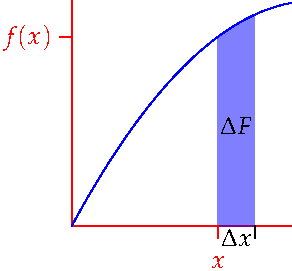
\includegraphics{ftcold}
\end{minipage}\smallbreak

In fact when Leibniz introduced the symbols $\int$ and $\D$ in the late 1600's, it was partly to reflect the fundamental theorem.\footnote{\def\dF{\D F}$\int$ is a stylized S for \emph{sum,} while $\D$ stands for \emph{difference.} Given a sequence $F=(F_0,F_1,F_2,\ldots,F_n)$, construct a new sequence of \emph{differences}
\[\dF=(F_1-F_0,F_2-F_1,\ldots,F_n-F_{n-1})\]
which can then be summed:
\[\int\dF=(F_1-F_0)+(F_2-F_1)+\cdots (F_n-F_{n-1})=F_n-F_0 \tag{$\ast$}\]
Viewing a function as an `infinite sequence' of values spaced along an interval, $\dF$ becomes a sequence of \emph{infinitesimals} and $(\ast)$ is essentially the fundamental theorem: $\int\dF =F(b)-F(a)$. It is the conception of a function that is suspect here, not the essential relationship between sums and differences.} If you're happy with non-rigorous notions of limit, rate of change, area, and (infinite) sums, the above is all you need!\smallbreak
Of course, we are very much concerned with the details: What must we assume regarding $f$ and $F$, and how are these properties used in the proof?

\begin{thm}{FTC, part I}{ftc1}
Suppose $f$ is integrable on $[a,b]$. For any $x\in[a,b]$, define
\[F(x):=\int_a^xf(t)\,\dt\]
Then:
\begin{enumerate}
  \item $F$ is uniformly continuous on $[a,b]$;
  \item If $f$ is continuous at $c\in[a,b]$, then $F$ is differentiable at $c$ with $F'(c)=f(c)$.
\end{enumerate}
\end{thm}

As ever, the condition at $c=a$ should be \emph{right}-continuous and the conclusion \emph{right}-differentiable, etc.\smallbreak
Compare this with the naïve version above where we assumed $f$ was continuous. We now require only the \emph{integrability} of $f$, and its continuity at \emph{one point} for the full result.\goodbreak



\begin{examples}{}{ftc1}
You should have seen many examples in an elementary calculus course.
\begin{enumerate}
  \item Since $f(x)=\sin^2(x^3-7)$ is continuous on any bounded interval, we conclude that
  \[\displaystyle\diff x\int_4^x\sin^2(t^3-7)\,\dt=\sin^2(x^3-7)\]
  If one follows Theorem \ref{thm:domainsplit} and its resulting conventions, then this is valid for all $x\in\R$.
  
  \item The chain rule permits more complicated examples. For instance, since $f(t)=\sin\sqrt t$ is continuous on its domain $[0,\infty)$ and $y(x)=x^2+3$ has range $[3,\infty)\subseteq\dom(f)$, we have
  \[\diff x\int_0^{x^2+3}\sin\sqrt t\,\dt =\diff[y]{x}\diff y\int_0^{y}\sin\sqrt t\,\dt=2x\sin\sqrt{x^2+3}\]
  
  \item For a final positive example, observe that
  \[\displaystyle \diff x\int_{\sin x}^{e^x} \tan(t^2)\,\dt =e^x\tan(e^{2x}) -\cos x\tan(\sin^2\!x)\]
  To evaluate this, one first chooses any constant $a$ and writes
  \[\int_{\sin x}^{e^x} =\int_a^{e^x}+\int_{\sin x}^a =\int_a^{e^x}-\int_a^{\sin x}\]
  before differentiating. This is valid provided $\sin x$, $e^x$ and $a$ all lie in the same subinterval of
  \[\dom\tan(t^2)=\R\setminus\{\pm\sqrt{\tfrac\pi 2},\pm\sqrt{\tfrac{3\pi}2},\pm\sqrt{\tfrac{5\pi}2},\ldots\}\]
  Since $\nm{\sin x}\le 1<\sqrt{\frac\pi 2}$, this requires
  \[\nm{e^{2x}}<\frac\pi 2 \iff x<\frac 12\ln\frac\pi 2\]
  Choosing $a=1$ would certainly suffice.
  
  \begin{minipage}[t]{0.7\linewidth}\vspace{0pt}
  \item\label{ex:ftcdiscont} Now consider why the theorem requires continuity. The piecewise continuous function
  \[f:[0,2]\to\R:x\mapsto\begin{cases}
  2x&\text{if }x\le 1\\
  \frac 12&\text{if }x>1
  \end{cases}\]
  has a jump discontinuity at $x=1$. We can still compute
  \[F(x)=\begin{cases}
  \int_0^x 2t\,\dt=x^2&\text{if }x\le 1\\
  \int_0^12t\,\dt+\int_1^x\frac 12\dt=\frac 12(x+1)&\text{if }x>1
  \end{cases}\]
  This is continuous, indeed uniformly so. However the discontinuity of $f$ results in $F$ having a \emph{corner} and thus being \emph{non-differentiable} at $x=1$. Indeed, $F'(x)=f(x)$ for all $x\neq 1$; that is, at all values of $x$ where $f$ is continuous.
  \end{minipage}\begin{minipage}[t]{0.3\linewidth}\vspace{0pt}
  \flushright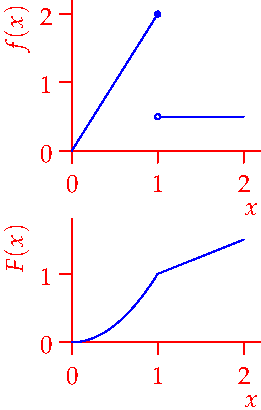
\includegraphics{ftc1}
  \end{minipage}
\end{enumerate}
\end{examples}
\vfil\goodbreak

\boldinline{Proving FTC\,I} Neither half of the theorem is particularly difficult once you write down what you know and what you need to prove. Here are the key ingredients:
\begin{enumerate}
  \item $F$ uniformly continuous means controlling the size of
  \[\nm{F(y)-F(x)}=\nm{\int_a^yf(t)\,\dt-\int_a^xf(t)\,\dt}=\nm{\int_x^yf(t)\,\dt}\le \int_x^y\nm{f(t)}\,\dt\]
  But the boundedness of $f$ allows us to bound this last integral\ldots
  \item $F'(c)=f(c)$ means showing that $\lim\limits_{x\to c}\frac{F(x)-F(c)}{x-c}=f(c)$, which means controlling the size of
  \[\nm{\frac{F(x)-F(c)}{x-c}-f(c)} =\nm{\frac 1{x-c}\int_{c}^xf(t)\,\dt-f(c)}\]
  The trick here will be to bring the \emph{constant} $f(c)$ inside the integral as $\frac 1{x-c}\int_c^xf(c)\,\dt$ so that what we really have to control is the size of $\frac 1{\nm{x-c}}\int_c^x\nm{f(t)-f(c)}\,\dt$. This is where the continuity of $f$ comes in\ldots
\end{enumerate}

\begin{proof}%[Proof of FTC\,I]
\begin{enumerate}
  \item Since $f$ is integrable, it is bounded: $\exists M>0$ such that $\nm{f(x)}\le M$ for all $x$.\smallbreak
	Let $\epsilon>0$ be given and define $\delta=\frac{\epsilon}M$. Then, for any $x,y\in[a,b]$,
	\begin{align*}
		0<y-x<\delta \implies \nm{F(y)-F(x)}&=\nm{\int_x^yf(t)\,\dt}\le \int_x^y\nm{f(t)}\,\dt \tag{Theorem \ref{thm:intineq}, part 4}\\
		&\le M(y-x) \tag{Theorem \ref{thm:intineq}, part 2}\\
		&<M\delta=\epsilon
	\end{align*}
	We conclude that $F$ is uniformly continuous on $[a,b]$.
	\item Let $\epsilon>0$ be given. Since $f$ is continuous at $c$, $\exists\delta>0$ such that, for all $t\in[a,b]$,
	\[\nm{t-c}<\delta \implies \nm{f(t)-f(c)}<\frac\epsilon 2\]
	Now for all $x\in[a,b]$ (except $c$),
	\begin{align*}
		0<\nm{x-c}<\delta\implies 
		&\nm{\frac{F(x)-F(c)}{x-c}-f(c)} =\nm{\frac 1{x-c}\int_{c}^xf(t)-f(c)\,\dt} \tag{Theorem \ref{thm:intlinear}}\\
		&\qquad\qquad\le\frac 1{\nm{x-c}}\int_{c}^x\nm{f(t)-f(c)}\dt \tag{Theorem \ref{thm:intineq}}\\
		&\qquad\qquad\le\frac 1{\nm{x-c}}\frac\epsilon 2\nm{x-c}=\frac\epsilon 2<\epsilon
	\end{align*}
	Clearly $\lim\limits_{x\to c}\frac{F(x)-F(c)}{x-c}=f(c)$, and so $F$ is differentiable at $c$ with $F'(c)=f(c)$.\qedhere
\end{enumerate}
\end{proof}

\vfil\goodbreak

\boldinline{The Fundamental Theorem, part II}

As with part I, the \emph{formulaic} part of the result should be familiar, though we are more interested in the assumptions and where they are needed.

\begin{thm}{FTC, part II}{ftc2}
Suppose $g$ is continuous on $[a,b]$, differentiable on $(a,b)$, and that $g'$ is integrable\footnotemark on $(a,b)$. Then,
\[\int_a^bg'=g(b)-g(a)\]
\end{thm}

\footnotetext{See Definition \ref{defn:intopen} if you're unsure what it means for $g'$ to be integrable on a bounded \emph{open} interval.}




Part II is often expressed in terms of \emph{anti-derivatives}: $F$ being an anti-derivative of $f$ if $F'=f$. Combined with \hyperref[thm:ftc1]{FTC\,I}, we recover the familiar `$+c$' result and a simpler version of the fundamental theorem often seen in elementary calculus.


\begin{cor}{}{}
Let $f$ be continuous on $[a,b]$.
\begin{itemize}
  \item If $F$ is an anti-derivative of $f$, then $\int_a^bf=F(b)-F(a)$.
  \item Every anti-derivative has the form $F(x)=\int_a^xf(t)\,\dt+c$ for some constant $c$.
\end{itemize}
\end{cor}



\begin{examples}{}{ftc2}
Again, basic examples should be familiar.
\begin{enumerate}
  \item Plainly $g(x)=x^2+2x^{3/2}$ is continuous on $[1,4]$ and differentiable on $(1,4)$ with derivative $g'(x)=2x+3\sqrt x$; this last is continuous (and thus integrable) on $(1,4)$. We conclude that
  \[\int_1^42x+3\sqrt x\,\dx =x^2+2x^{3/2}\Big|_1^4 =(16+16)-(1+2)=29\] 
  
  \item If $g(x)=\sin(3x^2)$, then $g'(x)=6x\cos(3x^2)$. Certainly $g$ satisfies the hypotheses of the theorem on any bounded interval $[a,b]$. We conclude
	\[\int_a^b 6x\cos(3x^2)\,\dx=\sin(3b^2)-\sin(3a^2)\]
	Moreover, every anti-derivative of $f(x)=6x\cos(3x^2)$ has the form $F(x)=\sin(3x^2)+c$.
	
	\item\label{ex:ftcdiscont2} Recall Example \hyperref[ex:ftcdiscont]{\ref*{ex:ftc1}.\ref*{ex:ftcdiscont}} where we saw that the discontinuity of $f$ led to the \emph{non-differentiability} of $F(x)=\int_0^xf(t)\,\dt$ at $x=1$. The function $F$ therefore fails the hypotheses of FTC\,II on the interval $[0,2]$.\smallbreak
	However, except at $x=1$, $F$ is an anti-derivative of $f$ and moreover $\int_0^2f(x)\,\dx=F(2)-F(0)$, so we \emph{appear} to have the formulaic conclusion of FTC\,II, though this is tautological given the definition of $F$!\smallbreak
	The way out of  this conundrum is to note that other anti-derivatives $\hat F$ of $f$ exist (except at $x=1$), and which fail to satisfy the conclusion. For instance
	  \[\hat F(x)=\begin{cases}
	  x^2&\text{if }x<1\\
	  \frac 12x&\text{if }x>1
	  \end{cases}\implies \hat F(2)-\hat F(0)=1\neq \frac 32=\int_0^2f(x)\,\dx\]
\end{enumerate}
\end{examples}


\goodbreak

\boldinline{Proving FTC\,II}

See Exercise \ref{ex:ftceasy} for a relatively easy proof when $g'=f$ is continuous. For the real McCoy, we can only rely on the \emph{integrability} of $g'$: the trick is to use the mean value theorem to write $g(b)-g(a)$ as a Riemann sum over a suitable partition.

\begin{proof}
Let $\epsilon>0$ be given and choose a partition $P$ such that $U(g',P)-L(g',P)<\epsilon$. Since $g$ satisfies the mean value theorem on each subinterval of the partition $P$, we see that
\[\exists \xi_i\in(x_{i-1},x_i)\quad\text{such that} \quad g'(\xi_i)=\frac{g(x_i)-g(x_{i-1})}{x_i-x_{i-1}}\]
from which
\[g(b)-g(a)=\sum_{i=1}^ng(x_i)-g(x_{i-1})=\sum_{i=1}^ng'(\xi_i)(x_i-x_{i-1})\]
This is a Riemann sum for $g'$ associated to the partition $P$, hence,
\[L(g',P)\le g(b)-g(a)\le U(g',P)\]
However we also have $L(g',P)\le \int_a^bg'\le U(g',P)$. Since these hold for all $\epsilon$, the proof is complete.
\end{proof}

While we certainly used the integrability of $g'$ in the proof, it might seem strange that we assumed it at all: shouldn't every derivative be integrable? Perhaps surprisingly, the answer is no! If you want a challenge, look up the \href{https://en.wikipedia.org/wiki/Volterra's_function}{\emph{Volterra function}}, which is differentiable everywhere, but whose derivative is \emph{non-integrable} (on, for instance, $[0,1]$)!


\boldsubsection{The Rules of Integration}

If one wants to \emph{evaluate} an integral, rather than merely show it exists, there are really only two options:
\begin{enumerate}
  \item Evaluate Riemann sums and take limits: often difficult if not impossible to do explicitly.
  \item Use \hyperref[thm:ftc2]{FTC\,II}. The problem now becomes the finding of \emph{anti-derivatives,} for which the core method is essentially \emph{guess and differentiate.} To obtain general rules, we attempt to reverse the rules of differentiation.
\end{enumerate}



\boldinline{Integration by Parts}

First consider the product rule: the product $g=uv$ of two differentiable functions is differentiable with $g'=u'v+uv'$.
Now apply Theorems \ref{thm:intlinear}, \ref{thm:intineq} and \hyperref[thm:ftc2]{FTC\,II}.

\begin{cor}{Integration by Parts}{}
Suppose $u,v$ are continuous on $[a,b]$, differentiable on $(a,b)$, and that $u',v'$ are integrable on $(a,b)$. Then
\[\int_a^bu'(x)v(x)\dx=u(b)v(b)-u(a)v(a)-\int_a^bu(x)v'(x)\dx\]
\end{cor}

This is significantly less useful than the product rule since it is only capable of transforming the integral of a product into another such integral.
\goodbreak

\begin{examples}{}{}
You should have seen myriad examples in a previous course. With practice, there is no need to explicitly state $u$ and $v$.
\begin{enumerate}
  \item Let $u(x)=x$ and $v'(x)=\cos x$. Then $u'(x)=1$ and $v(x)=\sin x$, whence
	\begin{align*}
		\int_0^{\pi/2} x\cos x\,\dx &=\left[x\sin x\right]_0^{\pi/2} -\int_0^{\pi/2}\sin x\,\dx =\frac\pi 2\sin\frac{\pi}2-0-\left[-\cos x\right]_0^{\pi/2}\\
		&=\frac\pi 2+\cos\frac\pi 2-\cos 0=\frac\pi 2-1
	\end{align*}
	\item Let $u(x)=\ln x$ and $v'(x)=1$. Then $u'(x)=\frac 1x$ and $v(x)=x$, whence
	\begin{align*}
		\int_e^{e^2} \ln x\,\dx &=\left[x\ln x\right]_e^{e^2} -\int_e^{e^2}\frac xx\,\dx =e^2\ln e^2-e\ln e-\left[x\right]_e^{e^2}\\
		&=2e^2-e-e^2+e =e^2
	\end{align*}
\end{enumerate}
\end{examples}

\boldinline{Change of Variables/Substitution}

We now turn our attention to the chain rule. If $g(x)=F\bigl(u(x)\bigr)$, where $F$ and $u$ are differentiable, then $g$ is differentiable with
\[g'(x)=\diff[g]{x}=\diff[F]{u}\diff[u]{x}=F'\bigl(u(x)\bigr) u'(x)\]
Now integrate both sides; the only issue is what assumptions are needed to invoke \hyperref[thm:ftc2]{FTC\,II}.

\begin{thm}{Substitution Rule}{intsubs}
Suppose we have two continuous functions: $u:[a,b]\to\R$ and $f:\range(u)\to\R$. Suppose also that $u$ is differentiable on $(a,b)$ with integrable derivative $u'$. Then
\[\int_a^bf\bigl(u(x)\bigr)\,u'(x)\,\dx=\int_{u(a)}^{u(b)}f(u)\,\du\]
\end{thm}

This is the famous `$u$-sub' formula from elementary calculus.

 
% \begin{proof}
% Given our hypotheses, we leave as an exercise the verification that both integrals exist. 
% % Since $f\circ u$ is continuous on $[a,b]$, it is also integrable. By Theorem \ref{thm:intineq}, $(f\circ u)u'$ is integrable on $[a,b]$, whence the left-hand integral exists. The right-hand integral exists since $f$ is continuous and thus integrable on $[u(a),u(b)]$ (or $[u(b),u(a)]$).
% Now fix $c\in I$ and define
% \[F(u):=\int_c^uf(t)\,\dt,\quad\forall u\in I\]
% Since $f$ is continuous, by \hyperref[thm:ftc1]{FTC\,I} we see that $F$ is differentiable on $I$ with $F'(u)=f(u)$. But now
% \begin{align*}
% \int_a^b f\bigl(u(x)\bigr)u'(x)\,\dx &=\int_a^b \left[\diff xF\bigl(u(x)\bigr)\right]\,\dx  \tag{chain rule}\\
% &= F\bigl(u(b)\bigr)-F\bigl(u(a)\bigr) \tag{FTC\,II}\\
% &=\int_{u(a)}^{u(b)}f(u)\,\du\tag*{\qedhere}
% \end{align*}
% \end{proof}

\begin{proof}
We leave as an exercise the verification that both integrals exist. We may also assume that $\range(u)$ is an interval of positive length\footnotemark for otherwise both integrals are trivially zero.\smallbreak
% Since $f\circ u$ is continuous on $[a,b]$, it is also integrable. By Theorem \ref{thm:intineq}, $(f\circ u)u'$ is integrable on $(a,b)$, whence the left-hand integral exists. The right-hand integral exists since $f$ is continuous on $\range(u)$ (note that this is a closed bounded interval since $u$ is continuous and $[a,b]$ is closed and bounded) and thus integrable on $[u(a),u(b)]$ (or $[u(b),u(a)]$).
Choose any $c\in\range(u)$ and define
\[F:\range(u)\to\R\ \text{ by }\ F(v):=\int_c^vf(t)\,\dt\]
Since $f$ is continuous, by \hyperref[thm:ftc1]{FTC\,I} we see that $F$ is differentiable with $F'(u)=f(u)$. But now
\begin{align*}
\int_a^b f\bigl(u(x)\bigr)u'(x)\,\dx &=\int_a^b \left[\diff xF\bigl(u(x)\bigr)\right]\,\dx  \tag{chain rule}\\
&= F\bigl(u(b)\bigr)-F\bigl(u(a)\bigr) \tag{FTC\,II}\\
&=\int_{u(a)}^{u(b)}f(u)\,\du\tag*{\qedhere}
\end{align*}
\end{proof}

\footnotetext{By the intermediate and extreme value theorems, $\range(u)$ is already a closed bounded interval.}


\begin{examples}{}{}
Reading the theorem is bad enough; its \emph{application} often requires significant creativity in order to recognize a suitable substitution.\footnotemark
\begin{enumerate}
  \item To evaluate the integral $\int_0^{\sqrt\pi}2x\sin x^2\,\dx$, consider the substitution $u(x)=x^2$ defined on $[0,\sqrt\pi]$. Certainly $u$ is continuous, and its derivative $u'(x)=2x$ is integrable on $(0,\sqrt\pi)$. Finally $f(u)=\sin u$ is continuous on $\range(u)=[0,\pi]$. The hypotheses are satisfied, whence
  \[\int_0^{\sqrt\pi}2x\sin x^2\,\dx = \int_0^{\sqrt\pi} f\bigl(u(x)\bigr)u'(x)\,\dx =\int_0^\pi\sin u\,\du =-\cos u\Big|_0^\pi=2\]
	\item For the following integral with $f(u)=\frac 1{u^2+1}$, we make the substitution $u(x)=x^2-2$. Note that $u:[\sqrt 2,\sqrt 3]\to[0,1]$ and that $u'(x)=2x$ is integrable; moreover, $f(u)$ is continuous on $\range(u)=[0,1]$. We conclude that
\[\int_{\sqrt 2}^{\sqrt 3}\frac{2x}{x^4-4x^2+5}\,\dx=\int_{\sqrt 2}^{\sqrt 3}\frac{2x}{(x^2-2)^2+1}\,\dx= \int_0^1\frac{1}{u^2+1}\,\du =\arctan u\Big|_0^1=\frac\pi 4\]
	\item The hypotheses on $u$ really are all that is necessary. In particular, $u$ doesn't need to be left-/right-differentiable at the endpoints of $[a,b]$! For instance, with $f(u)=u^2$ and $u(x)=\sqrt x$ on $[0,4]$, we easily verify
	\[\frac 83=\int_0^4\frac 12\sqrt x\,\dx =\int_0^4\frac x{2\sqrt x}\,\dx =\int_0^4f\bigl(u(x)\bigr)u'(x)\,\dx=\int_0^2f(u)\,\du =\int_0^2u^2\,\du =\frac 83\]
	\item Sloppy use of the substitution rule might lead to utter nonsense. For instance, consider the `substitution' $u=x^2$ in the following:
	\[\int_{-1}^2\frac 1x\,\dx= \int_{-1}^2\frac 1{2x^2}2x\,\dx =\int_1^4\frac 1{2u}\,\du=\frac 12(\ln 4-\ln 1)=\ln 2\]
	Of course the left hand integral does not exist since $\frac 1x$ is undefined at $0\in(-1,2)$, so the conclusion is false. In the language of the substitution rule, $f(u)=\frac 1{2u}$ is not continuous on $\range(u)=[0,4]$: it is not even defined at $u=0$! You are very unlikely to make precisely this mistake since the first integral is so clearly undefined, but for more complicated functions\ldots
\end{enumerate}
\end{examples}

\footnotetext{Hence the old adage, ``Differentiation is a science; integration an art.'' To illustrate via an example, consider the function $f(x)=\tan(e^x\cos(3x^2)+4x^3)$. The product and chain rules allow one to explicitly compute the derivative
\[\smash{\diff[f]{x}=\frac 1{1+(e^x\cos(3x^2)+4x^3)^2}\left(e^x\cos(3x^2)-6xe^x\sin(3x^2)+12x^2\right)}\]
By contrast, the integration analogues (integration by parts/substitution) are essentially useless in attempting to find an \emph{explicit} anti-derivative facilitating the integration of the same function via FTC\,II; for instance, the integral
\[\smash{\int_0^1\tan(e^x\cos(3x^2)+4x^3)\,\dx}\]
is likely impossible to evaluate explicitly and can only be approximated (e.g.\ via Riemann sums).}

\clearpage


\begin{exercises}
\exstart Calculate the following limits:
\begin{enumerate}\setcounter{enumi}{1}
  \item[]\begin{enumerate}
    \item $\displaystyle\lim_{x\to 0}\frac 1x\int_0^xe^{t^2}\dt$ \qquad\text{(b) }$\displaystyle\lim_{h\to 0}\frac 1h\int_3^{3+h}e^{t^2}\dt$
  \end{enumerate}
  
  \item Let $f(t)=\begin{cases}
  0&\text{if }t<0\\
  t&\text{if }0\le t\le 1\\
  4&\text{if }t>1
  \end{cases}$
   \begin{enumerate}
    \item Determine the function $F(x)=\int_0^xf(t)\,\dt$.
    \item Sketch $F$. Where is $F$ continuous?
    \item Where is $F$ differentiable? Calculate $F'$ at the points of differentiability.
   \end{enumerate}
  
  \item Let $f$ be a continuous function on $\R$.
  \begin{enumerate}
    \item Define $F(x)=\int_{x-1}^{x+1}f(t)\,\dt$. Carefully show that $F$ is differentiable on $\R$ and compute $F'$.
    \item Repeat for the function $G(x)=\int_0^{\sin x}f(t)\,\dt$.
  \end{enumerate}
  
  \item Recall Examples \hyperref[ex:ftcdiscont]{\ref*{ex:ftc1}.\ref*{ex:ftcdiscont}} and \hyperref[ex:ftcdiscont2]{\ref*{ex:ftc2}.\ref*{ex:ftcdiscont2}}. Find all anti-derivatives $F$ of $f$ on $[0,1)\cup(1,2]$. How many satisfy $\int_0^2f(x)\,\dx=F(2)-F(0)$?
  
  \item Consider integration by parts. Plainly $\int_a^xu'(t)v(t)\,\dt$ is an anti-derivative of $u'(x)v(x)$ by FTC\,I: what does integration by parts say is another?

  \item Use change of variables to integrate $\int_0^1x\sqrt{1-x^2}\,\dx$
  
	\item Use integration by parts and the substitution rule to evaluate $\int_0^b\arcsin x\,\dx$ for any $b<1$.

  \item Use integration by parts to evaluate $\int_0^b x\arctan x\,\dx$for any $b>0$
  
  \item Check that the assumptions of int by subs guarantee that both integrals are well-defined (i.e. that $(f\circ u)u'$ and $f$ are integrable on the required intervals.

  
  \item\label{ex:ftceasy} We prove a simpler version of the fundamental theorem of calculus.
  \begin{enumerate}
    \item Suppose $f$ is continuous on $[a,b]$ and define $F(x)=\int_a^xf(t)\,\dt$. For any $c,x\in[a,b]$ where $c\neq x$, prove that
    \[m\le\frac{F(x)-F(c)}{x-c}\le M\]
    where $m,M$ are the maximum and minimum values of $f(t)$ on the closed interval bounded by $c,x$. Make sure to explain why $m,M$ exist, and use this to deduce that $F'(c)=f(c)$.
    \item Suppose $f$ is continuous on $[a,b]$ and that $F$ is any anti-derivative of $f$ on $a,b$ (that is, $F'=f$). Use part (a) and the mean value theorem to prove that $\int_a^bf(t)\,\dt=F(b)-F(a)$.
  \end{enumerate}
  
%   
%   \item Suppose $f$ is piecewise continuous except at $x=c\in(a,b)$ where it has a discontinuity. Define $F(x)=\int_a^xf(t)\,\dt$.
%   \begin{itemize}
%     \item If the $f$ has a \emph{removable} discontinuity at $x=c$, prove that $F$ is differentiable at $x=c$ with $F'(c)\neq f(c)$.
%     \item If $f$ has a \emph{jump} discontinuity at $x=c$, prove that $F$ is not differentiable at $x=c$. (Hard!!)
%   \end{itemize}
  
%   \item HARD! Consider $f(x)=\begin{cases}
%   0&\text{if }x\not\in\Q\\
%   \frac 1q&\text{if }x=\frac pq\text{ is rational in lowest terms}
%   \end{cases}$
%   This function is continuous only on the irrationals. Prove that $f$ is integrable on any bounded interval $[a,b]$ and that $\int_a^bf=0$.

\end{enumerate}
\end{exercises}
\vfil
\goodbreak

\setcounter{subsection}{35}
\subsection{Improper Integrals}\label{sec:improper}

The Riemann integral has several limitations. Even allowing for functions to be integrable on open intervals (Exercise \hyperref[exs:extensionlemma]{\ref*{sec:riemann}.\ref*{exs:extensionlemma}}), the definition of $\int_a^bf(x)\,\dx$ requires the following:
\begin{itemize}
  \item That $(a,b)$ be a \emph{bounded} interval.
  \item That $f$ be \emph{bounded} on $(a,b)$.
\end{itemize}
There is a natural way to extend the Riemann integral to unbounded intervals and functions: \emph{limits.}

\begin{defn}{}{}
Suppose $f:[a,b)\to\R$ satisfies the following properties:
\begin{itemize}
  \item $f$ is integrable on every closed bounded subinterval $[a,t]\subseteq [a,b)$.
  \item Either $b=\infty$, or $b$ is finite and $f$ is unbounded at $b$,
\end{itemize}
The \emph{improper integral} of $f$ on $[a,b)$ is defined to be
\[\int_a^bf(x)\,\dx:=\lim_{t\to b^-}\int_a^tf(x)\,\dx\]
This is \emph{convergent} or \emph{divergent} in the same manner as the limit.\smallbreak
If an integral is improper at its lower limit then $\int_a^bf(x)\,\dx:=\lim\limits_{s\to a^+}\int_s^bf(x)\,\dx$.\smallbreak
If an integral is improper at both ends, choose any $c\in(a,b)$ and define
\[\int_a^bf(x)\,\dx =\lim_{s\to a^+}\int_s^cf(x)\,\dx+\lim_{t\to b^-}\int_c^tf(x)\,\dx\]
provided \emph{both} one-sided improper integrals exist and the limit sum makes sense.
\end{defn}

Theorem \ref{thm:domainsplit} says that the choice of $c$ for a doubly-improper integral is irrelevant.\medbreak

Many properties of the Riemann integral transfer to improper integrals, though not all. For example, part 1 of Theorem \ref{thm:intineq} extends:

\begin{thm}{}{impcomp}
If $0\le f(x)\le g(x)$ on $[a,b)$, then $\int_a^bf\le\int_a^bg$, whenever the integrals exist (standard or improper). In particular:
\begin{itemize}\itemsep2pt\parsep2pt
  \item $\int_a^bf=\infty\implies\int_a^bg=\infty$
  \item $\int_a^bg$ converges $\implies \int_a^bf$ converges to a value $\le \int_a^bg$.
\end{itemize}
\end{thm}
We leave some of the detail to Exercise \hyperref[ex:impropercomp]{\ref*{sec:improper}.\ref*{ex:impropercomp}}.

\vfil\pagebreak

\begin{examples}{}{improper}
\exstart $\int_0^tx^2\,\dx=\frac 13t^3$ for any $t>0$. Clearly
\[\int_0^\infty x^2\,\dx=\lim\limits_{t\to\infty}\frac 13t^3=\infty\]
More formally, the improper integral $\int_0^\infty x^2\,\dx$ diverges to infinity.

\begin{enumerate}\setcounter{enumi}{1}
  \item With $f(x)=x^{-4/3}$ defined on $[1,\infty)$,
  \[\int_1^\infty x^{-4/3}\,\dx=\lim_{t\to\infty}\int_1^tx^{-4/3}\,\dx =\lim_{t\to\infty}\left[-3x^{-1/3}\right]_1^t =\lim_{t\to\infty}3-3t^{-1/3} =3\]
  
  \item\label{ex:riemannsmotiv} Consider $f(x)=\nm xe^{-x^2/2}$ on $(-\infty,\infty)$. On a bounded interval $[0,t)$, we have
  \[\int_0^tf(x)\,\dx =\int_0^txe^{-x^2/2}\,\dx =\left[-e^{-x^2/2}\right]_0^t =1-e^{-t^2/2} \xrightarrow[t\to\infty]{} 1\]
  By symmetry, we conclude that
  \[\int_{-\infty}^\infty \nm xe^{-x^2/2}\,\dx=1+1=2\]
  This example is important in probability: multiplying by $\frac 1{\sqrt{2\pi}}$, we have computed the the expectation of $\nm{X}$ when $X$ is a normally-distributed random variable
  \[\E(\nm X)=\int_{-\infty}^\infty \frac 1{\sqrt{2\pi}}\nm xe^{-x^2/2}\,\dx=\sqrt{\frac 2\pi}\]
  
  \item If $t\in[0,1)$, we can use our knowledge of derivatives $\diff x\sin^{-1}x=\frac 1{\sqrt{1-x^2}}$ to evaluate
%   \footnote{If you've forgotten your derivatives, you can also do this by substitution.
%   \[x(u)=\sin u\implies \diff[x]{u}=\cos u=\sqrt{1-\sin^2\!u}=\sqrt{1-x^2} \implies \diff[u]{x}=\frac 1{\sqrt{1-x^2}}\]
%   where we take the positive square root since $x\in[0,1)$ is increasing. In the language of Theorem \ref{thm:intsubs}, $f(u)=1$ and so
%   \[\int_0^t\frac 1{\sqrt{1-x^2}}\,\dx= \int_0^{\sin^{-1}t}\,\du =\sin^{-1}t\]}
  \[\int_0^1\frac 1{\sqrt{1-x^2}}\,\dx=\lim_{t\to 1^-}\int_0^t\frac 1{\sqrt{1-x^2}}\,\dx=\lim_{t\to 1^-}\sin^{-1}t=\frac\pi 2\]
  and that, moreover $\int_{-1}^1\frac 1{\sqrt{1-x^2}}\,\dx=\pi$. By comparison, we see that
  \[\frac 1{\sqrt{1-x^4}}\le \frac 1{\sqrt{1-x^2}}\implies\int_{-1}^1\frac 1{\sqrt{1-x^4}}\,\dx\le \int_{-1}^1\frac 1{\sqrt{1-x^2}}\,\dx=\pi\]
  
  \item Improper integrals need not exist. For instance,
  \[\lim_{t\to\infty}\int_0^t\sin x\,\dx=\lim_{t\to\infty}1-\cos t\]
  diverges by oscillation.
\end{enumerate}
\end{examples}

\vfil\vfil\pagebreak

\begin{exercises}
\exstart Use your answers from the previous section to decide whether the improper integrals $\int_0^1\arcsin x\,\dx$ and $\int_0^\infty x\arctan x\,\dx$ exist. If so, what are their values?
\begin{enumerate}\setcounter{enumi}{1}
 	\item Let $p$ be a positive constant. Prove the following:
  \[\int_0^1\frac 1{x^p}\,\dx=\begin{cases}
  \frac 1{1-p}&\text{if }p<1\\
  \infty&\text{if }p\ge 1
  \end{cases}
  \qquad\qquad
  \int_1^\infty\frac 1{x^p}\,\dx=\begin{cases}
  \frac 1{p-1}&\text{if }p>1\\
  \infty&\text{if }p\le 1
  \end{cases}\]
  
  \goodbreak
  
  \item Explain why $\int_a^bf(x)\,\dx=\lim\limits_{t\to b^-}\int_a^tf(x)\,\dx$ holds, even when $f$ is integrable on $[a,b]$.  
  
  \item State a version of integration by parts modified for when $\int_a^b u'(x)v(x)\,\dx$ is an improper integral. Now evaluate $\int_0^\infty xe^{-4x}\,\dx$.
  
  \item What is wrong with the following calculation?
  \[\int_{-\infty}^\infty x\,\dx=\lim_{t\to\infty}\tfrac 12x^2\Big|_{-t}^t =\lim_{t\to\infty}\tfrac 12(t^2-t^2) =\lim_{t\to\infty}0=0\]
  
	\item Prove or disprove: if $\int f$ and $\int g$ are convergent improper integrals, so is $\int fg$.
  
  \item\label{ex:impropercomp} Prove part of Theorem \ref{thm:impcomp}. Suppose $0\le f(x)\le g(x)$ for all $x\in[a,b)$, and that $\int_a^bg$ is a convergent improper integral. Prove that $\int_a^bf$ converges and that $\int_a^bf\le\int_a^bg$.

  
  
%   
%   \item Suppose $f$ is piecewise continuous except at $x=c\in(a,b)$ where it has a discontinuity. Define $F(x)=\int_a^xf(t)\,\dt$.
%   \begin{itemize}
%     \item If the $f$ has a \emph{removable} discontinuity at $x=c$, prove that $F$ is differentiable at $x=c$ with $F'(c)\neq f(c)$.
%     \item If $f$ has a \emph{jump} discontinuity at $x=c$, prove that $F$ is not differentiable at $x=c$. (Hard!!)
%   \end{itemize}
  
%   \item HARD! Consider $f(x)=\begin{cases}
%   0&\text{if }x\not\in\Q\\
%   \frac 1q&\text{if }x=\frac pq\text{ is rational in lowest terms}
%   \end{cases}$
%   This function is continuous only on the irrationals. Prove that $f$ is integrable on any bounded interval $[a,b]$ and that $\int_a^bf=0$.

\end{enumerate}
\end{exercises}

\clearpage

\boldsubsection{Generalizing the Riemann Integral (non-examinable)}

In the 1890's, Thomas Stieltjes\footnote{Stieltjes was Dutch; for the pronunciation try `steelchez.'} offered a generalization of the Riemann integral.

\begin{defn}{}{}
Let $\alpha$ be a monotonically increasing function on an interval $[a,b]$. Given a partition $P=\{x_0,\ldots,x_n\}$ of $[a,b]$ and a function $f$, define the differences
\[\Delta\alpha_i=\alpha(x_i)-\alpha(x_{i-1})\]
The \emph{upper/lower Darboux--Stieltjes sums/integrals} are defined analogously to the pure Riemann case:\vspace{-5pt}
\begin{align*}
&U(f,P,\alpha)=\sum_{i=1}^n M_i\Delta\alpha_i\qquad &&L(f,P,\alpha)=\sum_{i=1}^n m_i\Delta\alpha_i &&\phantom{bobobobobobobobo}\\
&U(f,\alpha)=\inf U(f,P,\alpha)\qquad &&L(f,\alpha)=\sup L(f,P,\alpha)&&
\end{align*}
$f$ is \emph{Riemann--Stieltjes integrable} of class $\cR(\alpha)$ if $U(f,\alpha)=L(f,\alpha)$: we denote this value $\int_a^b f(x)\,\D\alpha$. 
\end{defn}

The standard Riemann integral corresponds to $\alpha(x)=x$. It is the ability to choose other functions $\alpha$ that makes the Riemann--Stieltjes integral both powerful and applicable. %Here are some properties and applications of the generalized integral.

\begin{description}
	\item[\normalfont\emph{Standard Properties}] Most results in sections \ref{sec:riemann} and \ref{sec:riemannproperties} hold with suitable modifications, as does the discussion of improper integrals. For instance,
  \[f\in\cR(\alpha) \iff \exists P\text{ such that }U(f,P,\alpha)-L(f,P,\alpha)<\epsilon\]
  The result regarding piecewise continuity of $f$ is a notable exception: if $f$ and $\alpha$ are simultaneously piecewise continuous then $f$ might not lie in $\cR(\alpha)$.
  	
	\item[\normalfont\emph{Weighted integrals}] If $\alpha$ is differentiable, then we obtain a standard Riemann integral
  \[\int_a^bf(x)\,\D\alpha =\int_a^bf(x)\alpha'(x)\,\dx\]
  weighted so that $f(x)$ contributes more when $\alpha$ is increasing rapidly. 
  
  \goodbreak
  
  \item[\normalfont\emph{Probability}] If $\alpha(a)=0$ and $\alpha(b)=1$, then $\alpha$ may be viewed as a \emph{probability distribution function.}%\footnote{When $[a,b]$ is finite, the convention in probability is to extend $\alpha$ to $\R$ via $\alpha(x)=0$ if $x\le a$ and $\alpha(x)=1$ if $x\ge b$: then all integrals can be taken over $\R$.}
  Its derivative $\alpha'$ is the corresponding \emph{probability density function.} For example:
  \begin{enumerate}
    \item The \emph{uniform distribution} on $[a,b]$ has $\alpha=\frac 1{b-a}(x-a)$ so that
    \[\int_a^bf(x)\,\D\alpha =\frac 1{b-a}\int_a^bf(x)\,\dx\] 
    Since $\alpha'$ is constant, the integrals weigh all values of $x$ \emph{uniformly.}
    \item The standard \emph{normal distribution} has $\alpha(x)=\int_{-\infty}^x\frac 1{\sqrt{2\pi}}e^{-t^2/2}\,\dt$. The fact that $\alpha'=\frac 1{\sqrt{2\pi}}e^{-x^2/2}$ is maximal when $x=0$ reflects the fact that a normally distributed variable is clustered near its mean.
  \end{enumerate}
  In all cases, $\int f(x)\,\D\alpha=\E(f(X))$ computes an expectation (see, for instance, Example \hyperref[ex:riemannsmotiv]{\ref*{ex:improper}.\ref*{ex:riemannsmotiv}}).
  
  \goodbreak

	\item[\normalfont\emph{Non-differentiable $\alpha$}] A major flexibility comes when we allow $\alpha$ to be non-differentiable, or even discontinuous! For example, given a partition $Q=\{s_0,\ldots,s_n\}$ of $[a,b]$, and a positive sequence $(c_k)_{k=1}^n$, define
  \[\alpha(x)=\begin{cases}
  0&\text{if }x=a\\
  \sum\limits_{i=1}^kc_i&\text{if }x\in (s_{k-1},s_{k}]
  \end{cases}\]
 	This is an increasing step function on $[a,b]$. The Riemann--Stieltjes integral becomes a weighted sum
%  	 For the partition $Q$, we have $\Delta\alpha_k=c_k$. Moreover, for any refinement $P$ of $Q$ any additional $\Delta\alpha_k$ are zero(!) and we have
%   \[U(f,P,\alpha) =\sum_{i=1}^{n}M_ic_i\qquad L(f,P,\alpha) =\sum_{i=1}^{n}m_ic_i\]
%   where $M_i,m_i$ are defined on each subinterval of the refinement $P$. If $f$ is continuous, in the limit we obtain $M_i,m_i\to f(s_i)$, etc., and 
  \[\int_a^bf(x)\,\D\alpha =\sum_{i=1}^nc_if(s_i)\]
  Taking instead an infinite sequence $(s_n)\subseteq[a,b]$ results in an infinite series, which helps explain why so many results for series and integrals look similar!\smallbreak
  This also touches on probability. For example, let $p\in[0,1]$, $n\in\N$, and $s_k=k$ on the interval $[0,n]$. If $c_k=\binom nkp^k(1-p)^{n-k}$, then
  \[\int f(x)\,\D\alpha =\sum_{k=0}^n\binom nkp^k(1-p)^{n-k} f(x)=\E(f(X))\]
  is the expectation of $f(X)$ when $X\sim B(n,p)$ is a binomially distributed random variable.
%   A similar analysis can be done with infinite sequences $(s_n)$ lying in $[a,b]$, thus unifying the concepts of integral and (infinite) sum. For example, if $s_n=1-\frac 1n$ and $c_n=\frac 1{n^2}$, then
%   \[\int_0^1x^2\,\D\alpha =\sum_{n=1}^\infty\frac 1{n^2}\left(1-\frac 1n\right)^2\]
  %is a convergent infinite series!
\end{description}

\goodbreak

\boldsubsubsection{Integrals and Convergence}

The \emph{Lebesgue integral} is another common generalization. Its main purpose is to permit the transfer of integrability to the limit of a sequence of integrable functions.\footnote{Recall how \emph{uniform convergence} does this for continuity.} To see the problem, consider the sequence
\[f_n:[0,1]\to\R:x\mapsto\begin{cases}
1&\text{if }x=\frac pq\in\Q\text{ with }q\le n\\
0&\text{otherwise}
\end{cases}\]
Each $f_n$ is piecewise continuous and thus Riemann integrable with $\int_0^1f_n(x)\,\dx=0$. However, the pointwise limit of $f_n$ is the function
\[f(x)=\begin{cases}
1&\text{if }x\in\Q\\
0&\text{if }x\not\in\Q
\end{cases}\]
which is \emph{not} Riemann integrable. In the Lebesgue theory, the limit $f$ turns out to be integrable with integral 0, so that
\[\lim_{n\to\infty}\int_0^1f_n(x)\,\dx=\int_0^1\lim_{n\to\infty}f_n(x)\,\dx\]
Recall that the interchange of limits and integrals would be automatic \emph{if} the convergence $f_n\to f$ were \emph{uniform}: of course the convergence isn't uniform here. 